\section*{16. Inference about Independence}\label{inference-about-independence}
This chapter addresses two questions:
\begin{enumerate}[tightlist,label={\arabic*.}]
\item
  How do we test if two random variables are independent?
\item
  How do we estimate the strength of dependence between two random
  variables?
\end{enumerate}
Recall we write \(Y \ci Z\) to mean that \(Y\) and \(Z\) are
independent.
When \(Y\) and \(Z\) are not independent, we say they are
\textbf{dependent} or \textbf{associated} or \textbf{related}.
Note that dependence does not mean causation: - Smoking is related to
heart disease, and quitting smoking will reduce the chance of heart
disease. - Owning a TV is related to lower starvation, but giving a
starving person a TV does not make them not hungry.

\subsection*{16.1 Two Binary Variables}\label{two-binary-variables}
Suppose that both \(Y\) and \(Z\) are binary. Consider a data set
\((Y_{1}, Z_{1}), \dots, (Y_{n}, Z_{n})\). Represent the data as a two-by-two
table:
\[
\begin{array}{c|cc|c} 
      & Y = 0  & Y = 1 & \\
\hline
Z = 0 & X_{00} & X_{01} & X_{0\text{·}}\\
Z = 1 & X_{10} & X_{11} & X_{1\text{·}}\\
 \hline
      & X_{\text{·}0} & X_{\text{·}1} & n = X_{\text{··}}
\end{array}
\]
where \(X_{ij}\) represents the number of observations where
\((Z_{k}, Y_{k}) = (i, j)\). The dotted subscripts denote sums,
e.g.~\(X_{i\text{·}} = \sum_{j} X_{ij}\). Denote the corresponding
probabilities by:
\[
\begin{array}{c|cc|c} 
      & Y = 0  & Y = 1 & \\
\hline
Z = 0 & p_{00} & p_{01} & p_{0\text{·}}\\
Z = 1 & p_{10} & p_{11} & p_{1\text{·}}\\
 \hline
      & p_{\text{·}0} & p_{\text{·}1} & 1
\end{array}
\]
where \(p_{ij} = \PROB(Z = i, Y = j)\). Let
\(X = (X_{00}, X_{01}, X_{10}, X_{11})\) denote the vector of counts.
Then \(X \sim \text{Multinomial}(n, p)\) where
\(p = (p_{00}, p_{01}, p_{10}, p_{11})\).
The \textbf{odds ratio} is defined to be
\[
\psi = \frac{p_{00} p_{11}}{p_{01} p_{10}}
\]
The \textbf{log odds ratio} is defined to be
\[
\gamma = \log \psi
\]

\textbf{Theorem 16.2}. The following statements are equivalent:
\begin{enumerate}[tightlist,label={\arabic*.}]
\item
  \(Y \ci Z\)
\item
  \(\psi = 1\)
\item
  \(\gamma = 0\)
\item
  For \(i, j \in \{ 0, 1 \}\), \(p_{ij} = p_{i\text{·}} p_{\text{·}j}\)
\end{enumerate}
Now consider testing
\[
H_{0}: Y \ci Z
\quad \text{versus} \quad
H_{1}: \text{not} (Y \ci Z)
\]
First consider the likelihood ratio test. Under \(H_{1}\),
\(X \sim \text{Multinomial}(n, p)\) and the MLE is \(\hat{p} = X / n\).
Under \(H_{0}\), again \(X \sim \text{Multinomial}(n, p)\) but \(p\) is
subjected to the constraint \(p_{ij} = p_{i.} p_{.j}\). This leads to
the following test.

\textbf{Theorem 16.3 (Likelihood Ratio Test for Independence in a 2-by-2
table)}. Let
\[
T = 2 \sum_{i=0}^{1} \sum_{j=0}^{1} X_{ij} \log \left( \frac{X_{ij} X_{\text{··}}}{X_{i\text{·}} X_{\text{·}j}} \right)
\]
Under \(H_{0}\), \(T \leadsto \chi_{1}^{2}\). Thus, an approximate level
\(\alpha\) test is obtained by rejecting \(H_{0}\) when
\(T > \chi_{1, \alpha}^{2}\).

\textbf{Theorem 16.4 (Pearson's \(\chi^{2}\) test for Independence in a
2-by-2 table)}. Let
\[
U = \sum_{i=0}^{1} \sum_{j=0}^{1} \frac{(X_{ij} - E_{ij})^{2}}{E_{ij}}
\]
where
\[
E_{ij} = \frac{X_{i\text{·}} X_{\text{·}j}}{n}
\]
Under \(H_{0}\), \(U \leadsto \chi_{1}^{2}\). Thus, an approximate level
\(\alpha\) test is obtained by rejecting \(H_{0}\) when
\(U > \chi_{1, \alpha}^{2}\).
Here is the intuition for the Pearson test: Under \(H_{0}\),
\(p_{ij} = p_{i\text{·}} p_{\text{·}j}\), so the MLE of \(p_{ij}\) is
\(\hat{p}_{ij} = \hat{p}_{i\text{·}} \hat{p}_{\text{·}j} = \frac{X_{i\text{·}}}{n} \frac{X_{\text{·}j}}{n}\).
Thus, the expected number of observations in the \((i, j)\) cell is
\(E_{ij} = n \hat{p}_{ij} = \frac{X_{i\text{·}} X_{\text{·}j}}{n}\). The
statistic \(U\) compares the observed and expected counts.

\textbf{Theorem 16.6}. The MLEs of \(\psi\) and \(\gamma\) are
\[
\hat{\psi} = \frac{X_{00} X_{11}}{X_{01} X_{10}}
, \quad
\hat{\gamma} = \log \hat{\psi}
\]
The asymptotic standard errors (computed from the delta method) are
\begin{align*}
\widehat{\SE}(\hat{\psi}) &= \sqrt{\frac{1}{X_{00}} + \frac{1}{X_{01}} + \frac{1}{X_{10}} + \frac{1}{X_{11}}}\\
\widehat{\SE}(\hat{\gamma}) &= \hat{\psi} \widehat{\SE}(\hat{\gamma})
\end{align*}
Yet another test of independence is the Wald test for \(\gamma = 0\)
given by \(W = (\hat{\gamma} - 0) / \widehat{\SE}(\hat{\gamma})\).
A \(1 - \alpha\) confidence interval for \(\gamma\) is
\(\hat{\gamma} \pm z_{\alpha/2} \widehat{\SE}(\hat{\gamma})\).
A \(1 - \alpha\) confidence interval for \(\psi\) can be obtained in two
ways. First, we could use
\(\hat{\psi} \pm z_{\alpha/2} \widehat{\SE}(\hat{\psi})\). Second,
since \(\psi = e^{\gamma}\) we could use
\(\exp \{\hat{\gamma} \pm z_{\alpha/2} \widehat{\SE}(\hat{\gamma})\}\).
This second method is usually more accurate.

\subsection*{16.2 Interpreting the Odds
Ratios}\label{interpreting-the-odds-ratios}
Suppose event \(A\) has probability \(\PROB(A)\). The odds of \(A\)
are defined as
\[
\text{odds}(A) = \frac{\PROB(A)}{1 - \PROB(A)}
\]
It follows that
\[
\PROB(A) = \frac{\text{odds}(A)}{1 + \text{odds}(A)}
\]
Let \(E\) be the event that someone is exposed to something (smoking,
radiation, etc) and let \(D\) be the event that they get a disease. The
odds of getting the disease given exposure are:
\[
\text{odds}(D | E) = \frac{\PROB(D | E)}{1 - \PROB(D | E)}
\]
and the odds of getting the disease given non-exposure are:
\[
\text{odds}(D | E^{c}) = \frac{\PROB(D | E^{c})}{1 - \PROB(D | E^{c})}
\]
The \textbf{odds ratio} is defined to be
\[
\psi = \frac{\text{odds}(D | E)}{\text{odds}(D | E^{c})}
\]
If \(\psi = 1\) then the disease probability is the same for exposed and
unexposed; this implies these events are independent. Recall that the
log-odds ratio is defined as \(\gamma = \log \psi\). Independence
corresponds to \(\gamma = 0\).
Consider this table of probabilities:
\[
\begin{array}{c|cc|c} 
      & D^{c}    & D      & \\
\hline
E^{c}   & p_{00} & p_{01} & p_{0\text{·}}\\
E     & p_{10} & p_{11} & p_{1\text{·}}\\
 \hline
      & p_{\text{·}0} & p_{\text{·}1} & 1
\end{array}
\]
Denote the data by
\[
\begin{array}{c|cc|c} 
      & D^{c}    & D      & \\
\hline
E^{c}   & X_{00} & X_{01} & X_{0\text{·}}\\
E     & X_{10} & X_{11} & X_{1\text{·}}\\
 \hline
      & X_{\text{·}0} & X_{\text{·}1} & X_{\text{··}}
\end{array}
\]
Now
\[
\PROB(D | E) = \frac{p_{11}}{p_{10} + p_{11}}
\quad \text{and} \quad
\PROB(D | E^{c}) = \frac{p_{01}}{p_{00} + p_{01}}
\]
and so
\[
\text{odds}(D | E) = \frac{p_{11}}{p_{10}}
\quad \text{and} \quad
\text{odds}(D | E^{c}) = \frac{p_{01}}{p_{00}}
\]
and therefore
\[
\psi = \frac{p_{11}p_{00}}{p_{01}p_{10}}
\]
To estimate the parameters, we have to consider how the data were
collected. There are three methods.
\textbf{Multinomial Sampling}. We draw a sample from the population and, for each sample, record their exposure and disease status. In this case, 
\(X = (X_{00}, X_{01}, X_{10}, X_{11}) \sim \text{Multinomial}(n, p)\). 
We then estimates the probabilities in the table by 
\(\hat{p}_{ij} = X_{ij} / n\) and
\[
\hat{\psi} = \frac{\hat{p}_{11} \hat{p}_{00}}{\hat{p}_{01} \hat{p}_{10}} = \frac{X_{11} X_{00}}{X_{01} X_{10}}
\]
\textbf{Prospective Sampling (Cohort Sampling)}. We get some exposed and
unexposed people and count the number with disease within each group.
Thus,
\[
X_{01} \sim \text{Binomial}(X_{0\text{·}}, \PROB(D | E^{c}))
\quad \text{and} \quad
X_{11} \sim \text{Binomial}(X_{1\text{·}}, \PROB(D | E))
\]
In this case we should write small letters
\(x_{0\text{·}},  x_{1\text{·}}\) instead of capital letters $
X_{0\placeholder}, X_{1\placeholder}$ since they are fixed and not
random, but we'll keep using capital letters for notational simplicity.
We can estimate \(\PROB(D | E))\) and \(\PROB(D | E^{c})\) but
we cannot estimate all probabilities in the table. Still, we can
estimate \(\psi\). Now:
\[
\hat{\PROB}(D | E) = \frac{X_{11}}{X_{1\text{·}}}
\quad \text{and} \quad
\hat{\PROB}(D | E^{c}) = \frac{X_{01}}{X_{0\text{·}}}
\]
Thus,
\[
\hat{\psi} = \frac{X_{11} X_{00}}{X_{01} X_{10}}
\]
as before.
\textbf{Case-Control (Retrospective Sampling)}. Here we get some
diseased and non-diseased people and we observe how many are exposed.
This is much more efficient if the disease is rare. Hence,
\[
X_{10} \sim \text{Binomial}(X_{\text{·}0}, \PROB(E | D^{c}))
\quad \text{and} \quad
X_{11} \sim \text{Binomial}(X_{\text{·}1}, \PROB(E | D))
\]
From this data we can estimate \(\PROB(E | D)\) and
\(\PROB(E | D^{c})\). Surprisingly, we can still estimate \(\psi\).
To understand why, note that
\[
\PROB(E | D) = \frac{p_{11}}{p_{01} + p_{11}},
\quad 1 - \PROB(E | D) = \frac{p_{01}}{p_{01} + p_{11}},
\quad \text{odds}(E | D) = \frac{p_{11}}{p_{01}}
\]
By a similar argument,
\[
\text{odds}(E | D^{c}) = \frac{p_{10}}{p_{00}}
\]
Hence,
\[
\frac{\text{odds}(E | D)}{\text{odds}(E | D^{c})} = \frac{p_{11} p_{00}}{p_{01} p_{10}} = \psi
\]
Therefore,
\[
\hat{\psi} = \frac{X_{11} X_{00}}{X_{01} X_{10}}
\]
In all three methods, the estimate of \(\psi\) turns out to be the same.
It is tempting to try to estimate
\(\PROB(D | E) - \PROB(D | E^{c})\). In a case-control design,
this quantity is not estimable. To see this, we apply Bayes' Theorem to
get
\[
\PROB(D | E) - \PROB(D | E^{c}) = \frac{\PROB(E | D) \PROB(D))}{\PROB(E)} - \frac{\PROB(E^{c} | D) \PROB(D)}{\PROB(E^{c})}
\]
Because of the way we obtained the data, \(\PROB(D)\) is not
estimable from the data.
However, we can estimate
\(\xi = \PROB(D | E) / \PROB(D | E^{c})\), which is called the
\textbf{relative risk}, under the \textbf{rare disease assumption}.

\textbf{Theorem 16.9}. Let
\(\xi = \PROB(D | E) / \PROB(D | E^{c})\). Then
\[
\frac{\psi}{\xi} \rightarrow 1
\]
as \(\PROB(D) \rightarrow 0\).
Thus, under the rare disease assumption, the relative risk is
approximately the same as the odds ratio, which we can estimate.
In a randomized experiment, we can interpret a strong association, that
is \(\psi \neq 1\), as a causal relationship. In an observational
(non-randomized) study, the association can be due to other unobserved
\textbf{confounding} variables. We'll discuss causation in more detail
later.

\subsection*{16.3 Two Discrete
Variables}\label{two-discrete-variables}
Now suppose that \(Y \in \{ 1, \dots, I \}\) and
\(Z \in \{ 1, \dots, J \}\) are two discrete variables. The data can be
represented by an \(I \times J\) table of contents:
    \[
\begin{array}{c|cccccc|c} 
       & Y = 1  & Y = 2  & \cdots & Y = j & \cdots & Y = J   & \\
\hline
Z = 1 & X_{11}  & X_{12} & \cdots & X_{1j} & \cdots & X_{1J} & X_{1\text{·}}\\
Z = 2 & X_{21}  & X_{22} & \cdots & X_{2j} & \cdots & X_{2J} & X_{2\text{·}}\\
\vdots & \vdots & \vdots & \vdots & \vdots & \vdots & \vdots & \vdots\\
Z = i & X_{i1}  & X_{i2} & \cdots & X_{ij} & \cdots & X_{iJ} & X_{i\text{·}}\\
\vdots & \vdots & \vdots & \vdots & \vdots & \vdots & \vdots & \vdots\\
Z = I & X_{I1}  & X_{I2} & \cdots & X_{Ij} & \cdots & X_{IJ} & X_{I\text{·}}\\
 \hline
      & X_{\text{·}1} & X_{\text{·}1} & \cdots & X_{\text{·}j} & \cdots & X_{\text{·}J} & n
\end{array}
\]
Consider testing
\[
H_{0}: Y \ci Z
\quad \text{versus} \quad
H_{1}: \text{not } H_{0}
\]

\textbf{Theorem 16.10}. Let
\[
T = 2 \sum_{i=1}^I \sum_{j=1}^J X_{ij} \log \left( \frac{X_{ij} X_{\text{··}}}{X_{i\text{·}} X_{\text{·}j}} \right)
\]
The limiting distribution of \(T\) under the null hypothesis of
independence is \(\chi^{2}_\nu\) where \(\nu = (I - 1)(J - 1)\).
Pearson's \(\chi^{2}\) test statistic is
\[
U = \sum_{i=1}^I \sum_{j=1}^J \frac{(n_{ij} - E_{ij})^{2}}{E_{ij}}
\]
Asymptotically, under \(H_{0}\), \(U\) has a \(\chi^{2}_\nu\) distribution
where \(\nu = (I - 1)(J - 1)\).
There are a variety of ways to quantify the strength of dependence
between two discrete variables \(Y\) and \(Z\). Most of them are not
very intuitive. The one we shall use is not standard but is more
interpretable.
We define
\[
\delta(Y, Z) = \max_{A, B} \Big|\; \PROB_{Y, Z}(Y \in A, Z \in B) - \PROB_Y(Y \in A)\PROB_Z(Z \in B) \;\Big|
\]
where the maximum is over all pairs of events \(A\) and \(B\).
\emph{Note: the original version on the book contains a typo; it is
originally stated as}
\[
\delta(Y, Z) = \max_{A, B} \Big|\; \PROB_{Y, Z}(Y \in A, Z \in B) - \PROB_Y(Y \in A) - \PROB_Z(Z \in B) \;\Big|
\]
\emph{For more context, this is a specific case of the ``total variation
distance'' \(\delta(P_{1}, P_{2})\) between the probability metrics
\(P_{1}(Y, Z) = \PROB_{Y, Z}(Y \in A, Z \in B)\) and
\(P_{2}(Y, Z) = \PROB_Y(Y \in A)\PROB_Z(Z \in B)\).}

\textbf{Theorem 16.12}. Properties of \(\delta(Y, Z)\):
\begin{enumerate}[tightlist,label={\arabic*.}]
\item
  \(0 \leq \delta(Y, Z) \leq 1\)
\item
  \(\delta(Y, Z) = 0\) if and only if \(Y \ci Z\)
\item
  The following identity holds:
\end{enumerate}
\[
\delta(X, Y) = \frac{1}{2} \sum_{i=1}^I \sum_{j=1}^J \Big|\; p_{ij} - p_{i\text{·}} p_{\text{·}j} \;\Big|
\]
\begin{enumerate}[tightlist,label={\arabic*.},resume]
\item
  The MLE of \(\delta\) is
\end{enumerate}
\[
\hat{\delta}(X, Y) = \frac{1}{2} \sum_{i=1}^I \sum_{j=1}^J \Big|\; \hat{p}_{ij} - \hat{p}_{i\text{·}} \hat{p}_{\text{·}j} \;\Big|
\]
where
\[
\hat{p}_{ij} = \frac{X_{ij}}{n},
\quad \hat{p}_{i\text{·}} = \frac{X_{i\text{·}}}{n},
\quad \hat{p}_{\text{·}j} = \frac{X_{\text{·}j}}{n}
\]
The interpretation of \(\delta\) is this: if one person makes
probability statements assuming independence and another person makes
probability statements without assuming independence, their probability
statements may differ by as much as \(\delta\). Here is a suggested scale
for interpreting \(\delta\):
\begin{table}[H]
\centering
\begin{tabular}{@{}ll@{}}
\toprule
range & interpretation \\
\midrule
0 to 0.01 & negligible association \\
0.01 to 0.05 & non-negligible association \\
0.05 to 0.1 & substantial association \\
over 0.1 & very strong association \\
\bottomrule
\end{tabular}
\end{table}
A confidence interval for \(\delta\) can be obtained by bootstrapping.
The steps are:
\begin{enumerate}[tightlist,label={\arabic*.}]
\item
  Draw \(X^{*} \sim \text{Multinomial}(n, \hat{p})\);
\item
  Compute \(\hat{p}_{ij}, \hat{p}_{i\text{·}}, \hat{p}_{\text{·}j}\);
\item
  Compute \(\delta^{*}\);
\item
  Repeat.
\end{enumerate}
Now we use any of the methods we learned earlier for constructing
bootstrap confidence intervals. However, we should not use a Wald
interval in this case. The reason is that if \(Y\) and \(Z\) are
independent then \(\delta = 0\) and we are on the boundary of the
parameter space. In this case, the Wald method is not valid.

\subsection*{16.4 Two Continuous
Variables}\label{two-continuous-variables}
Now suppose that \(Y\) and \(Z\) are both continuous. If we assume that
the joint distribution of \(Y\) and \(Z\) is bivariate Normal, then we
measure the dependence between \(Y\) and \(Z\) by means of the
correlation coefficient \(\rho\). Tests, estimates, and confidence
intervals for \(\rho\) in the Normal case are given in the previous
chapter. If we do not assume normality, then we need a nonparametric
method for asserting dependence.
Recall that the correlation is
\[
\rho = \frac{\EXP((X_{1} - \mu_{1})(X_{2} - \mu_{2}))}{\sigma_{1} \sigma_{2}}
\]
A nonparametric estimator of \(\rho\) is the plug-in estimator which is:
\[
\hat{\rho} = \frac{\sum_{i=1}^{n} (X_{1i} - \bar{X}_{1})(X_{2i} - \bar{X}_{2})}{\sqrt{\sum_{i=1}^{n} (X_{1i} - \bar{X}_{1})^{2} \sum_{i=1}^{n} (X_{2i} - \bar{X}_{2})^{2}}}
\]
which is just the sample correlation. A confidence interval can be
constructed using the bootstrap. A test for \(\rho = 0\) can be based on
the Wald test using the bootstrap to estimate the standard error.
The plug-in approach is useful for large samples. For small samples, we
measure the correlation using the \textbf{Spearman rank correlation
coefficient} \(\hat{\rho}_S\). We simply replace the data by their
ranks, ranking each variable separately, then compute the correlation
coefficient of the ranks.
To test the null hypothesis that \(\rho_S = 0\), we need the
distribution of \(\hat{\rho}_S\) under the null hypothesis. This can be
obtained by simulation. We fix the ranks of the first variable as
\(1, 2, \dots, n\). The ranks of the second variable are chosen at
random from the set of \(n!\) possible orderings, then we compute the
correlation. This is repeated many times, and the resulting distribution
\(\PROB_{0}\) is the null distribution of \(\hat{\rho}_S\). The
p-value for the test is \(\PROB_{0}(|R| > |\hat{\rho}_S|)\) where
\(R\) is drawn from the null distribution \(\PROB_{0}\).

\subsection*{16.5 One Continuous Variable and One
Discrete}\label{one-continuous-variable-and-one-discrete}
Suppose that \(Y \in \{ 1, \dots, I \}\) is discrete and \(Z\) is
continuous. Let \(F_{i}(z) = \PROB(Z \leq z | Y = i)\) denote the CDF
of \(Z\) conditional on \(Y = i\).

\textbf{Theorem 16.15}. When \(Y \in \{ 1, 2, \dots, I \}\) is discrete
and \(Z\) is continuous, then \(Y \ci Z\) if and only if
\(F_{1} = F_{2} = \dots = F_I\).
It follows that to test for independence, we need to test
\[
H_{0}: F_{1} = \dots = F_I
\quad \text{versus} \quad
H_{1}: \text{not } H_{0}
\]
For simplicity, we consider the case where \(I = 2\). To test the null
hypothesis that \(F_{1} = F_{2}\) we will use the \textbf{two sample
Kolmogorov-Smirnov test}.
Let \(n_{k}\) denote the number of observations for which \(Y_{i} = k\). Let
\[
\hat{F}_{k}(z) = \frac{1}{n_{k}} \sum_{i=1}^{n} I(Z_{i} \leq z) I(Y_{i} = k)
\]
denote the empirical distribution function of \(Z\) given \(Y = k\).
Define the test statistic
\[
D = \sup_x | \hat{F}_{1}(x) - \hat{F}_{2}(x) |
\]

\textbf{Theorem 16.16}. Let
\[
H(t) = 1 - 2 \sum_{j=1}^{\infty} (-1)^{j-1} e^{-2j^{2}t^{2}}
\]
Under the null hypothesis that \(F_{1} = F_{2}\),
\[
\lim_{n \rightarrow \infty} \PROB \left( \sqrt{\frac{n_{1} n_{2}}{n_{1} + n_{2}}} D \leq t \right) = H(t)
\]
It follows from the Theorem than an approximate level \(\alpha\) test is
obtained by rejecting \(H_{0}\) when
\[
\sqrt{\frac{n_{1} n_{2}}{n_{1} + n_{2}}} D > H^{-1}(1 - \alpha)
\]

\subsection*{16.7 Exercises}

\textbf{Exercise 16.7.1}. Prove Theorem 16.2.
The following statements are equivalent:
\begin{enumerate}[tightlist,label={\arabic*.}]
\item
  \(Y \ci Z\)
\item
  \(\psi = 1\)
\item
  \(\gamma = 0\)
\item
  For \(i, j \in \{ 0, 1 \}\), \(p_{ij} = p_{i\text{·}} p_{\text{·}j}\)
\end{enumerate}

\textbf{Solution}.
\(Y\) and \(Z\) are independent if and only if
\(\PROB(Y = j | Z = i) = \PROB(Y = j) \PROB(Z = i)\) for
all \(i\) and \(j\), so (1) and (4) are equivalent.
\(\gamma = \log \psi\), so (2) and (3) are equivalent.
Finally,
\begin{align*}
&\psi = 1\\
&\Leftrightarrow \frac{\text{odds}(Y | Z = 1)}{\text{odds}(Y | Z = 0)} = 1 \\
&\Leftrightarrow \text{odds}(Y | Z = 1) = \text{odds}(Y | Z = 0) \\
&\Leftrightarrow \PROB(Y | Z = 1) = \PROB(Y | Z = 0) \\
&\Leftrightarrow Y \ci Z
\end{align*}
so (1) and (2) are equivalent.
Therefore, all statements are equivalent.

\textbf{Exercise 16.7.2}. Prove Theorem 16.3.
Let
\[
T = 2 \sum_{i=0}^{1} \sum_{j=0}^{1} X_{ij} \log \left( \frac{X_{ij} X_{\text{··}}}{X_{i\text{·}} X_{\text{·}j}} \right)
\]
Under \(H_{0}\), \(T \leadsto \chi_{1}^{2}\). Thus, an approximate level
\(\alpha\) test is obtained by rejecting \(H_{0}\) when
\(T > \chi_{1, \alpha}^{2}\).

\textbf{Solution}. Let
\(E_{ij} = \frac{X_{i\text{·}} X_{\text{·}j}}{X_\text{··}}\). We can
rewrite the test statistic as
\[
T = 2 \sum_{i, j} X_{ij} \log \frac{X_{ij}}{E_{ij}}
\]
The interpretation of \(E_{ij}\) is that it is the expected count in
cell \((i, j)\) under \(H_{0}\):
\begin{align*}
\EXP_{H_{0}}(Y = i, Z = j) &= n \PROB_{H_{0}}(Y = i, Z = j) \\
&= n \PROB(Y = i) \PROB(Z = j) \\
&= n \hat{p}_{i\text{·}} \hat{p}_{\text{·}j} \\
&= X_{\text{··}} \frac{X_{i\text{·}}}{X_{\text{··}}} \frac{X_{\text{·}j}}{X_{\text{··}}} \\
&= E_{ij}
\end{align*}
Now, the result will follow by applying the log-likelihood test between
\(H_{0}\) and \(H_{1}\). The test statistic is:
\[
2 \log \frac{\mathcal{L}(\tilde{p} | X)}{\mathcal{L}(\hat{p} | X)} 
= 2 \log \frac{\prod_{i, j} \tilde{p}_{ij}^{X_{ij}}}{\prod_{i, j} \hat{p}_{ij}^{X_{ij}}}
\]
where \(\tilde{p}\) is the MLE under \(H_{1}\) and \(\hat{p}\) is the MLE
under \(H_{0}\). But we have:
\[
\tilde{p}_{ij} = \frac{X_{ij}}{n}
\quad \text{and} \quad
\hat{p}_{ij} = \frac{E_{ij}}{n}
\]
Substituting the MLEs on the log-likelihood ratio, we get
\[
2 \log \frac{\mathcal{L}(\tilde{p} | X)}{\mathcal{L}(\hat{p} | X)} 
= 2 \log \prod_{i, j} \left( \frac{X_{ij}}{E_{ij}} \right)^{X_{ij}}
= 2 \sum_{i, j} X_{ij} \log \frac{X_{ij}}{E_{ij}}
\]
which is the desired result.
\emph{Reference: ``G-test.'' Wikipedia: The Free Encyclopedia. Wikimedia
Foundation, Inc.~22 July 2004. Web. 17 Mar.~2020,
en.wikipedia.org/w/index.php?title=G-test\&oldid=914538756}

\textbf{Exercise 16.7.3}. Prove Theorem 16.9.
Let \(\xi = \PROB(D | E) / \PROB(D | E^{c})\). Then
\[
\frac{\psi}{\xi} \rightarrow 1
\]
as \(\PROB(D) \rightarrow 0\).

\textbf{Solution}. We have:
\[
\PROB(D | E) = \frac{\PROB(D \land E)}{\PROB(E)} = \frac{p_{11}}{p_{01} + p_{11}}
\quad
\PROB(D | E^{c}) = \frac{\PROB(D \land E^{c})}{\PROB(E^{c})} = \frac{p_{10}}{p_{00} + p_{10}}
\]
and so
\[
\xi = \frac{\PROB(D | E)}{\PROB(D | E^{c})}
= \frac{p_{11} (p_{00} + p_{10})}{p_{10} (p_{01} + p_{11})}
\]
Since
\[
\psi = \frac{p_{11}p_{00}}{p_{01}p_{10}}
\]
we have:
\[
\frac{\psi}{\xi} = \frac{p_{11}p_{00}}{p_{01}p_{10}} \frac{p_{10} (p_{01} + p_{11})}{p_{11} (p_{00} + p_{10})} 
= \frac{p_{00}}{p_{01}} \frac{p_{\text{·}1}}{p_{\text{·}0}}
\]
As \(\PROB(D) = p_{10} + p_{11} \rightarrow 0\) and the
probabilites are non-negative, \(p_{10} \rightarrow 0\),
\(p_{11} \rightarrow 0\), so
\[
\frac{\psi}{\xi} \rightarrow  \frac{p_{00}}{p_{01}} \frac{p_{01}}{p_{00}} = 1
\]

\textbf{Exercise 16.7.4}. Prove equation (16.14).
\[
\delta(X, Y) = \max_{A, B} \Big|\; \PROB_{X, Y}(X \in A, Y \in B) - \PROB_X(X \in A) \PROB_Y(Y \in B) \;\Big|
\]
is equivalent to
\[
\delta(X, Y) = \frac{1}{2} \sum_{i=1}^I \sum_{j=1}^J \Big|\; p_{ij} - p_{i\text{·}} p_{\text{·}j} \;\Big|
\]

\textbf{Solution}.
As noted when the definition was introduced, this definition of
\(\delta(X, Y)\) is a particular case of the total variation distance
between metrics \(P_{1}(X, Y) = \PROB_{X, Y}(X \in A, Y \in B)\) and
\(P_{2}(X, Y) = \PROB_X(X \in A) \PROB_Y(Y \in B)\), where
\[
\delta(P, Q) = \sup_{A \in \mathcal{F}} |P(A) - Q(A)|
\]
and \(P, Q\) are two probability measures on a sigma-algebra
\(\mathcal{F}\) of subsets from the sample space \(\Omega\).
(Note that \(P_{1}(X = i, Y = j) = p_{ij}\) and
\(P_{2}(X = i, Y = j) =  p_{i\text{·}} p_{\text{·}j}\)).
It is a known property of the total variation distance in countable
spaces that
\[
\delta(P, Q) = \max_{A \in \mathcal{F}} |P(A) - Q(A)| = \frac{1}{2} \Vert P - Q \Vert_{1} = \frac{1}{2} \sum_{\omega \in \Omega} \vert P(\omega) - Q(\omega) \vert
\]
Demonstrate it, following the steps in the reference below.
Let \(\mathcal{F}^+ \subset \mathcal{F}\) be the set of states
\(\omega\) such that \(P(\omega) \geq Q(\omega)\), and let
\(\mathcal{F}^- = \mathcal{F} - S^+\) be the set of states \(\omega\)
such that \(P(\omega) < Q(\omega)\). We have:
\[
\max_{A \in \mathcal{F}} P(A) - Q(A) = P(\mathcal{F}^+) - Q(\mathcal{F}^+)
\]
and
\[
\max_{A \in \mathcal{F}} Q(A) - P(A) = Q(\mathcal{F}^-) - P(\mathcal{F}^-)
\]
But since \(P(\Omega) = Q(\Omega) = 1\), we have
\[
P(\mathcal{F}^+) + P(\mathcal{F}^-) = Q(\mathcal{F}^+) + Q(\mathcal{F}^-) = 1
\]
which implies that
\[
P(\mathcal{F}^+) - Q(\mathcal{F}^+) = Q(\mathcal{F}^-) - P(\mathcal{F}^-)
\]
hence
\[
\max_{A \in \mathcal{F}} P(A) - Q(A) = \vert P(\mathcal{F}^+) - Q(\mathcal{F}^+) \vert = \vert Q(\mathcal{F}^-) - P(\mathcal{F}^-) \vert
\]
Finally, since
\[
\vert P(\mathcal{F}^+) - Q(\mathcal{F}^+) \vert + \vert Q(\mathcal{F}^-) - P(\mathcal{F}^-) \vert = \sum_{\omega \in \Omega} | P(\omega) - Q(\omega) | = \Vert P - Q \Vert_{1}
\]
we have that
\[
\max_{A \in \mathcal{F}} |P(A) - Q(A)| = \frac{1}{2} \Vert P - Q \Vert_{1}
\]
which completes the proof.
\emph{Reference: Upfal, E., and M. Mitzenmacher. ``Probability and
computing.'' (2005). Lemma 11.1, pg. 272-273.}

\textbf{Exercise 16.7.5}. The New York Times (January 8, 2003, page A12)
reported the following data on death sentencing and rance, from a study
in Maryland:
\begin{table}[H]
\centering
\begin{tabular}{@{}lll@{}}
\toprule
& Death Sentence & No Death Sentence \\
\midrule
Black Victim & 14 & 641 \\
White Victim & 62 & 594 \\
\bottomrule
\end{tabular}
\end{table}
Analyse the data using the tools from this Chapter. Interpret the
results. Explain why, based only on this information, you cannot make
causal conclusions. (The authors of the study did use much more
information in their full report).

\textbf{Solution}.
The statistic for the log-likelihood test for independence is is:
\[
T = 2 \sum_{i, j} X_{ij} \log \frac{X_{ij} X_{\text{··}}}{X_{i\text{·}} X_{\text{·}j}}
\]
The statistic for Pearson's \(\chi^{2}\) test is:
\[
U = \sum_{i, j} \frac{(X_{ij} - E_{ij})^{2}}{E_{ij}}
\]

\begin{python}
import numpy as np
X_ij = np.array([[14, 641], [62, 594]])
\end{python}

\begin{python}
X_idot = X_ij.sum(axis = 1).reshape(2, 1)
X_dotj = X_ij.sum(axis = 0).reshape(1, 2)
n = X_ij.sum()
E_ij = X_idot @ X_dotj / n
# Log-likelihood test statistic
T = 2 * (X_ij * np.log(X_ij / E_ij)).sum()
# Pearson's \chi^{2} test statistic
U = ((X_ij - E_ij)**2 / E_ij).sum()
\end{python}

\begin{python}
from scipy.stats import chi2
p_value_log_likelihood = 1 - chi2.cdf(T, 1)
p_value_pearson = 1 - chi2.cdf(U, 1)
print('T test statistic: \t\t%.3f'% T)
print('Pearson chi^{2} statistic: \t%.3f'% U)
print('p-value log likelihood:\t\t %.3f' % p_value_log_likelihood)
print('p-value Pearson: \t\t %.3f' % p_value_pearson)
\end{python}
\begin{console}
T test statistic:               34.534
Pearson chi^{2} statistic:        32.104
p-value log likelihood:          0.000
p-value Pearson:                 0.000
\end{console}
Both tests indicate that these variables are correlated. Note that this
is not sufficient information, in itself, to imply causation.

\begin{python}
from itertools import product
p = X_ij / n
p_idot = X_idot / n
p_dotj = X_dotj / n
delta = sum([abs(p[i, j] - p_idot[i, :] * p_dotj[:, j]) 
            for (i, j) in product(range(2), range(2))]) / 2
print('delta(X, Y): %.3f' % delta)
\end{python}
\begin{console}
delta(X, Y): 0.037
\end{console}
\(\delta(X, Y)\) is between 0.01 and 0.05, suggesting a non-negligible
association.

\textbf{Exercise 16.7.6}. Analyse the data on the variables Age and
Financial Status from:
\url{http://lib.stat.cmu.edu/DASL/Datafiles/montanadat.html}

\textbf{Solution}.

\begin{python}
import pandas as pd
data = pd.read_csv('data/montana.csv')
# Select wanted columns and remove missing data
data = data[['AGE', 'FIN']].replace('*', np.nan).dropna().astype(int)
\end{python}

\begin{python}
# Count occurrences in each cell
X_ij = np.zeros((3, 3)).astype(int)
for index, row in data.iterrows():
     X_ij[row['AGE'] - 1, row['FIN'] - 1] += 1
           
X_ij
\end{python}
\begin{console}
array([[21, 16, 34],
       [17, 23, 26],
       [22, 37, 11]])
\end{console}

\begin{python}
X_idot = X_ij.sum(axis = 1).reshape(3, 1)
X_dotj = X_ij.sum(axis = 0).reshape(1, 3)
n = X_ij.sum()
E_ij = X_idot @ X_dotj / n
# Log-likelihood test statistic
T = 2 * (X_ij * np.log(X_ij / E_ij)).sum()
# Pearson's \chi^{2} test statistic
U = ((X_ij - E_ij)**2 / E_ij).sum()
\end{python}

\begin{python}
from scipy.stats import chi2
p_value_log_likelihood = 1 - chi2.cdf(T, 4)
p_value_pearson = 1 - chi2.cdf(U, 4)
print('T test statistic: \t\t%.3f'% T)
print('Pearson chi^{2} statistic: \t%.3f'% U)
print('p-value log likelihood:\t\t %.3f' % p_value_log_likelihood)
print('p-value Pearson: \t\t %.3f' % p_value_pearson)
\end{python}
\begin{console}
T test statistic:               22.064
Pearson chi^{2} statistic:        20.679
p-value log likelihood:          0.000
p-value Pearson:                 0.000
\end{console}
Both tests indicate correlation between the two sequences.

\begin{python}
from itertools import product
p = X_ij / n
p_idot = X_idot / n
p_dotj = X_dotj / n
delta = sum([abs(p[i, j] - p_idot[i, :] * p_dotj[:, j]) 
            for (i, j) in product(range(3), range(3))]) / 2
print('delta(X, Y): %.3f' % delta)
\end{python}
\begin{console}
delta(X, Y): 0.128
\end{console}
\(\delta(X, Y) > 0.1\) indicates a strong correlation between these
variables.

\textbf{Exercise 16.7.7}. Estimate the correlation between temperature
and latitude using the data from
\url{http://lib.stat.cmu.edu/DASL/Datafiles/USTemperatures.html}
Use the correlation coefficient and Spearman rank correlation. Provide
estimates, tests, and confidence intervals.

\textbf{Solution}.

\begin{python}
import math
import numpy as np
import pandas as pd
data = pd.read_csv('data/USTemperatures.txt', sep='\t')
filtered_data = data[['lat', 'JanTF']].dropna()
X, Y = filtered_data['lat'], filtered_data['JanTF']
\end{python}

\begin{python}
from scipy.stats import rankdata
from tqdm import tqdm_notebook
def get_pearson_correlation(xx, yy):
    mu_1 = xx.mean()
    mu_2 = yy.mean()
    sigma2_1 = ((xx - mu_1)**2).mean()
    sigma2_2 = ((yy - mu_2)**2).mean()
    
    return ((xx - mu_1) * (yy - mu_2)).mean() / math.sqrt(sigma2_1 * sigma2_2)
def get_spearman_correlation(xx, yy):
    return get_pearson_correlation(rankdata(xx), rankdata(yy))
def bootstrap_correlation(xx, yy, corr_fun, B=10000, alpha=0.05):
    n = len(xx)
    assert len(yy) == n, 'Sequences must have same length'
    
    t_boot = np.empty(B)
    for i in tqdm_notebook(range(B)):
        indexes = np.random.randint(0, n, size=n)
        xx_selected, yy_selected = xx.iloc[indexes], yy.iloc[indexes]
        t_boot[i] = corr_fun(xx_selected, yy_selected)
        
    confidence_interval = (np.quantile(t_boot, alpha / 2), np.quantile(t_boot, 1 - alpha / 2))
    return confidence_interval
\end{python}

\begin{python}
pearson_rho = get_pearson_correlation(X, Y)
pearson_rho_confidence = bootstrap_correlation(X, Y, 
    corr_fun = get_pearson_correlation, B = 10000, alpha=0.05)
spearman_rho = get_spearman_correlation(X, Y)
spearman_rho_confidence = bootstrap_correlation(X, Y, 
    corr_fun = get_spearman_correlation, B = 10000, alpha=0.05)
\end{python}

\begin{python}
print('Pearson confidence: \t %.3f' % pearson_rho)
print('95%% confidence interval: %.3f, %.3f' % pearson_rho_confidence)
print()
print('Spearman confidence: \t %.3f' % spearman_rho)
print('95%% confidence interval: %.3f, %.3f' % spearman_rho_confidence)
\end{python}
\begin{console}
Pearson confidence:      -0.857
95\% confidence interval: -0.964, -0.684
Spearman confidence:     -0.834
95\% confidence interval: -0.953, -0.649
\end{console}

\textbf{Exercise 16.7.8}. Test whether calcium intake and drop in blood
pressure are associated. Use the data in
\url{http://lib.stat.cmu.edu/DASL/Datafiles/Calcium.html}

\textbf{Solution}.
We intend to use Theorem 16.16 here:
Let
\[
H(t) = 1 - 2 \sum_{j=1}^{\infty} (-1)^{j-1} e^{-2j^{2}t^{2}}
\]
Under the null hypothesis that \(F_{1} = F_{2}\),
\[
\lim_{n \rightarrow \infty} \PROB \left( \sqrt{\frac{n_{1} n_{2}}{n_{1} + n_{2}}} D \leq t \right) = H(t)
\]
where
\[
D = \sup_x | \hat{F}_{1}(x) - \hat{F}_{2}(x) |
\]
It follows from the Theorem than an approximate level \(\alpha\) test is
obtained by rejecting \(H_{0}\) when
\[
\sqrt{\frac{n_{1} n_{2}}{n_{1} + n_{2}}} D > H^{-1}(1 - \alpha)
\]

\begin{python}
import pandas as pd
import matplotlib.pyplot as plt
data = pd.read_csv('data/calcium.txt', sep='\t')
X, Y = data['Treatment'], data['Decrease']
\end{python}

\begin{python}
plt.figure(figsize=(12, 8))
plt.hist(data[data['Treatment'] == 'Placebo']['Decrease'], 
         density=True, bins=50, color='red', label='Placebo')
plt.hist(data[data['Treatment'] == 'Calcium']['Decrease'], 
         density=True, bins=50, color='blue', label='Calcium')
plt.legend(loc='upper right')
plt.show()
\end{python}

\begin{figure}[H]
\centering
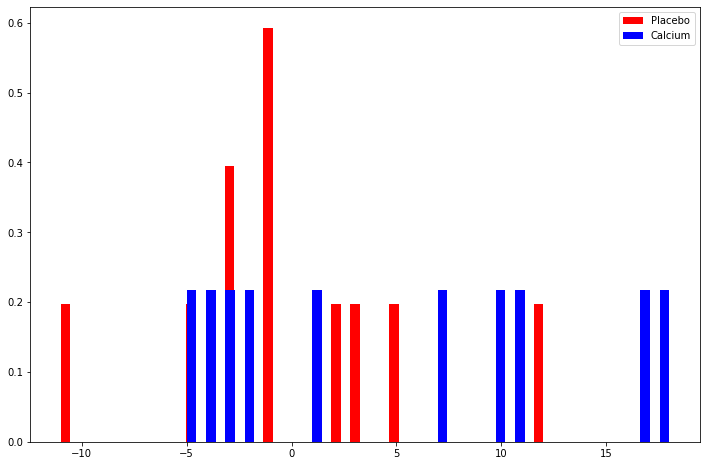
\includegraphics{Figure-16-01}
\end{figure}

First,  calculate D -- creating the empirical CDFs \(\hat{F}_{1}\)
and \(\hat{F}_{2}\), and then testing the value of \(D\) for each possible
\(x\) in the empirical distributions:

\begin{python}
f1 = data[data['Treatment'] == 'Placebo']['Decrease'].to_numpy()
f2 = data[data['Treatment'] == 'Calcium']['Decrease'].to_numpy()
def f1_hat(x):
    return sum(f1 <= x) / len(f1)
def f2_hat(x):
    return sum(f2 <= x) / len(f2)
xx = np.linspace(min(data['Decrease']) - 1, max(data['Decrease']) + 1, 100)
fig, (ax1, ax2) = plt.subplots(2, sharex=True, figsize=(12, 8))
ax1.plot(xx, [f1_hat(x) for x in xx], color='blue', label='F1 empirical distribution')
ax1.plot(xx, [f2_hat(x) for x in xx], color='red', label='F2 empirical distribution')
ax1.legend(loc='upper left')
ax2.plot(xx, [abs(f1_hat(x) - f2_hat(x)) for x in xx], color='purple', label='|F1 - F2|')
ax2.legend(loc='upper left')
plt.show()
\end{python}

\begin{python}
D = max([abs(f1_hat(x) - f2_hat(x)) for x in data['Decrease']])
n1 = len(f1)
n2 = len(f2)
test_statistic = np.sqrt(n1 * n2 / (n1 + n2)) * D
print('D: %.3f' % D)
print('Test statistic: %.3f' % test_statistic)
\end{python}
\begin{console}
D: 0.409
Test statistic: 0.936
\end{console}
Given that
\begin{align*}
H(t) &= 1 - 2 \sum_{j=1}^{\infty} (-1)^{j-1} e^{-2j^{2}t^{2}}
\end{align*}
 create an approximation for \(H^{-1}(1 - \alpha)\) -- so that we
may find the p-value for \(\alpha\) such that $
\sqrt{\frac{n_{1} n_{2}}{n_{1} + n_{2}}} D > H^{-1}(1 -
\alpha) $.

\begin{python}
def H(t, xtol=1e-8):
    assert t != 0, "t must be non-zero"
    t2 = t * t
    j_max = int(np.ceil(np.sqrt(- np.log(xtol / 2) / (2 * t2) )))
    jj = np.arange(1, j_max+1)
    return 1 + 2 * sum((-1)**(jj) * np.exp(-2 * (jj**2) * t2))
\end{python}

\begin{python}
# Plot some values for H(t)
tt = np.logspace(-3, 0.25, 100)
ht = [H(t) for t in tt]
plt.figure(figsize=(6, 4))
plt.plot(tt, ht)
plt.title('H(t)')
plt.show()
\end{python}

\begin{figure}[H]
\centering
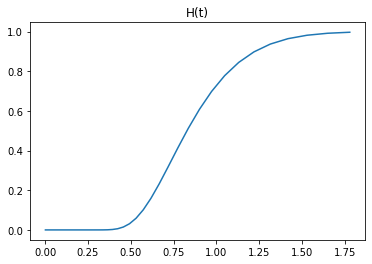
\includegraphics{Figure-16-03}
\end{figure}


\begin{python}
from scipy.optimize import minimize
def H_inv(q):
    def loss_function(x):
        return (H(x) - q)**2
    
    x0 = 1.0
    return minimize(loss_function, x0, method='nelder-mead').x
\end{python}

\begin{python}
# Plot some values for H_inv(q)
qq = np.linspace(1e-5, 1 - 1e-5, 200)
xx = [H_inv(q) for q in qq]
plt.figure(figsize=(6, 4))
plt.plot(qq, xx)
plt.title('H^{-1}(q)')
plt.show()
\end{python}

\begin{figure}[H]
\centering
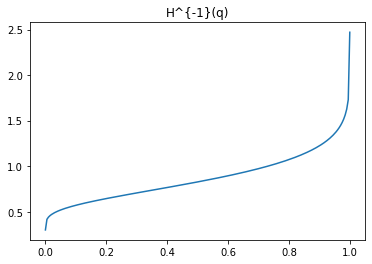
\includegraphics{Figure-16-04}
\end{figure}


\begin{python}
h_inv_test_statistic = H_inv(test_statistic)
print('Test statistic: \t\t%.3f' % test_statistic)
print('H^{-1}(test_statistic): \t%.3f' % h_inv_test_statistic)
\end{python}
\begin{console}
Test statistic:                 0.936
H^{-1}(test\_statistic):         1.313
\end{console}
Given that the inverse of the test statistic is greater than 1, we have
that the test from Theorem 16.16 rejects the null hypothesis for any
\(\alpha > 0\) -- so it claims the distributions are distinct at any
approximate \(\alpha\) level -- so, by Theorem 16.15, they are
associated.
